\subsection{Gleichstrommaschine}
	Die Gleichstrommascheine besteht im Stator entweder aus Permanetmagneten, oder aus einer permanent-erregten Erregerwicklung. Der Rotor besteht aus Wicklungen, welche durch einen Kommutator (auch Stromwender genannt) und B�rsten mithilfe von Gleichspannung versorgt werden. Die Drehzahl der Maschine kann hierbei ganz einfach durch Ver�ndern der Versorgungsspannung linear geregelt werden.\cite{Fischer2017}
	
	\begin{figure}[H]
			\centering
			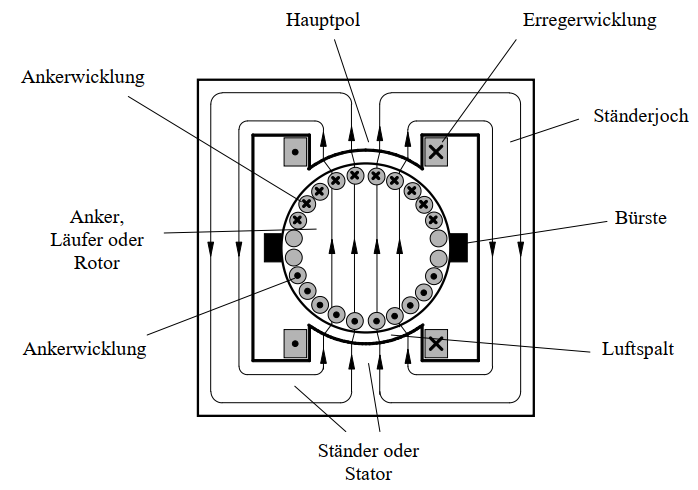
\includegraphics[scale=0.8]{./3_Stand_der_Technik/Abbildungen/Gleichstrommaschine_1}
			\caption{Aufbau Gleichstrommaschine\cite{Pischtschan2024}}
	\end{figure}
	
	Vorteil der Gleichstrommaschine ist die einfache Drehzahlregelung durch Ver�nderung der Spannung und relativ g�nstige Bauweise, da keine Frequenzumrichter n�tig ist. Zu den Nachteilen z�hlt der hohe Wartungsaufwand und Verschlei� der Maschine. Er wird aufgrund von sinkenden Preisen von Frequenzumrichtern immer weniger verwendet.